% Options for packages loaded elsewhere
\PassOptionsToPackage{unicode}{hyperref}
\PassOptionsToPackage{hyphens}{url}
%
\documentclass[
]{article}
\usepackage{amsmath,amssymb}
\usepackage{lmodern}
\usepackage{ifxetex,ifluatex}
\ifnum 0\ifxetex 1\fi\ifluatex 1\fi=0 % if pdftex
  \usepackage[T1]{fontenc}
  \usepackage[utf8]{inputenc}
  \usepackage{textcomp} % provide euro and other symbols
\else % if luatex or xetex
  \usepackage{unicode-math}
  \defaultfontfeatures{Scale=MatchLowercase}
  \defaultfontfeatures[\rmfamily]{Ligatures=TeX,Scale=1}
\fi
% Use upquote if available, for straight quotes in verbatim environments
\IfFileExists{upquote.sty}{\usepackage{upquote}}{}
\IfFileExists{microtype.sty}{% use microtype if available
  \usepackage[]{microtype}
  \UseMicrotypeSet[protrusion]{basicmath} % disable protrusion for tt fonts
}{}
\makeatletter
\@ifundefined{KOMAClassName}{% if non-KOMA class
  \IfFileExists{parskip.sty}{%
    \usepackage{parskip}
  }{% else
    \setlength{\parindent}{0pt}
    \setlength{\parskip}{6pt plus 2pt minus 1pt}}
}{% if KOMA class
  \KOMAoptions{parskip=half}}
\makeatother
\usepackage{xcolor}
\IfFileExists{xurl.sty}{\usepackage{xurl}}{} % add URL line breaks if available
\IfFileExists{bookmark.sty}{\usepackage{bookmark}}{\usepackage{hyperref}}
\hypersetup{
  pdftitle={R Markdown Documents - Part 1},
  pdfauthor={Amanda Klehr},
  hidelinks,
  pdfcreator={LaTeX via pandoc}}
\urlstyle{same} % disable monospaced font for URLs
\usepackage[margin=1in]{geometry}
\usepackage{graphicx}
\makeatletter
\def\maxwidth{\ifdim\Gin@nat@width>\linewidth\linewidth\else\Gin@nat@width\fi}
\def\maxheight{\ifdim\Gin@nat@height>\textheight\textheight\else\Gin@nat@height\fi}
\makeatother
% Scale images if necessary, so that they will not overflow the page
% margins by default, and it is still possible to overwrite the defaults
% using explicit options in \includegraphics[width, height, ...]{}
\setkeys{Gin}{width=\maxwidth,height=\maxheight,keepaspectratio}
% Set default figure placement to htbp
\makeatletter
\def\fps@figure{htbp}
\makeatother
\setlength{\emergencystretch}{3em} % prevent overfull lines
\providecommand{\tightlist}{%
  \setlength{\itemsep}{0pt}\setlength{\parskip}{0pt}}
\setcounter{secnumdepth}{-\maxdimen} % remove section numbering
\ifluatex
  \usepackage{selnolig}  % disable illegal ligatures
\fi

\title{R Markdown Documents - Part 1}
\usepackage{etoolbox}
\makeatletter
\providecommand{\subtitle}[1]{% add subtitle to \maketitle
  \apptocmd{\@title}{\par {\large #1 \par}}{}{}
}
\makeatother
\subtitle{Analysis of Environmental Data}
\author{Amanda Klehr}
\date{}

\begin{document}
\maketitle

{
\setcounter{tocdepth}{2}
\tableofcontents
}
\hypertarget{introduction}{%
\section{Introduction}\label{introduction}}

My name is \textbf{Amanda Klehr}. I typically go by \textbf{Mandy}, but
I answer to both! 
\includegraphics{assignments/cat_wink_small.jpg}

I just moved to Amherst from Portland, Oregon. I miss Portland a lot,
but I am really excited about continuing to pursue my \emph{Master of
Science} within the Department of Environmental Conservation in
wildlife, fish and conservation biology.

I started virtually in Spring 2021 and I really appreciate the chance to
be on campus and interact with my professors and cohorts in-person this
semester. Obviously, I love cats and I have one super cuddly, 11-year
old cat named Deirdre Daffodil Pottendorf, or DeeDee for short.

\hypertarget{concepts-list}{%
\section{Concepts List}\label{concepts-list}}

The things I would like to gain from this course include the following:

\begin{enumerate}
\def\labelenumi{\arabic{enumi}.}
\tightlist
\item
  R basics and techniques
\item
  Exploring different packages in R to use for modeling my data (e.g.,
  using for N-Mixture Models)
\item
  Using R Markdown to create documents like this one and presentations,
  etc. to design and communicate my results in an user-friendly manner
\item
  I like visuals and am also excited to learn more about creating tables
  and figures in R as well
\end{enumerate}

\hypertarget{course-list}{%
\section{Course List}\label{course-list}}

All of the courses I have taken at UMass so far have been great!
Including:

\begin{itemize}
\tightlist
\item
  Introduction to GIS
\item
  Offshore Wind Energy: Environmental Impacts, Siting, Permitting, and
  Stakeholder Engagement (wow - that's a mouthful!)\\
\item
  Clean Energy and Climate Change Policy in the Commonwealth of
  Massachusetts (also, quite the course title)
\item
  Analysis of Environmental Data: lecture and lab (foundational and so
  thrilled to be here!)
\end{itemize}

Also a shout out to a few courses from my undergrad at Portland State
University (10 years ago - eek!) that were stellar and are really the
reason I am here today:

\begin{itemize}
\tightlist
\item
  Vertebrate Zoology
\item
  Ornithology
\item
  Marine Mammalogy (and all of the other courses related to marine
  mammals I took from Dr.~Deb Duffield )
\end{itemize}

(You can tell I'm a wildlife person\ldots)

\hypertarget{bonus-deedee}{%
\section{Bonus: DeeDee}\label{bonus-deedee}}

Here is a cute image of DeeDee! 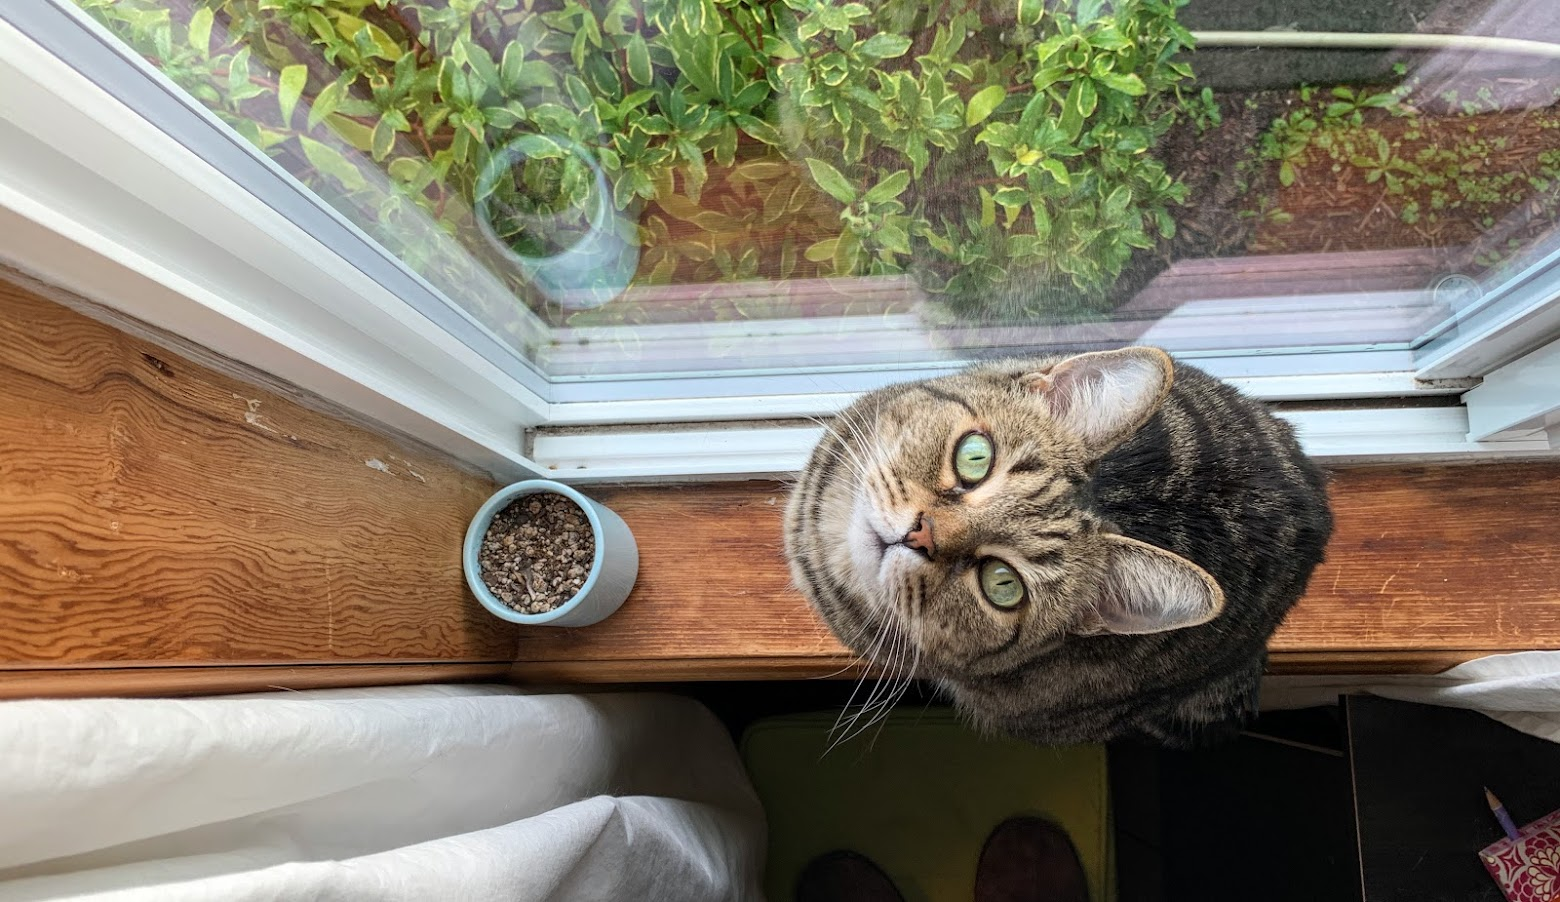
\includegraphics{assignments/dee.jpg}

\end{document}
